%%%%%%%%%%%%%%%%%%%%%%%%%%%%%%%%%%%%%%%%%%%%%%%%%%%%%%
%%%%%%%%%%%%%%%%%%%%%%%%%%%%%%%%%%%%%%%%%%%%%%%%%%%%%%%%%%%%%%%%%%%%
\def\scl{0.4}%scaling factor of the picture
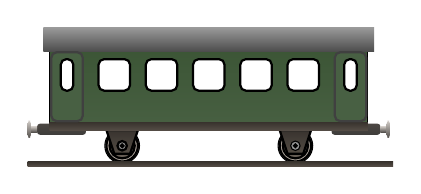
\begin{tikzpicture}[
  scale=\scl,
  %wagon/.style={yellow!30!brown!20!,rounded corners,draw=black,thick},
  wagon/.style={green!70!brown!20!black!75!,draw=black,thick},
 % toit/.style={black!70!brown!20!,draw=gray,thick},
  roue/.style={brown!20!black!70!,draw=black,thick},
  fenetre/.style={white,rounded corners = 2pt,draw=black, thick},
  porte/.style={green!70!brown!20!black!75!,rounded corners = 2pt,draw=gray!50!black, thick}
  ]
%
%      WAGON
%
  \begin{scope}[xshift=0 cm,yshift=0 cm]
  %\fill[wagon] (0.75, 1.25) rectangle (10.75, 3.75);
  \shade[bottom color=green!70!brown!20!black!75!, top color=green!70!brown!20!black!80!,draw=black,thin]
 (0.7, 1.25) rectangle (10.8, 3.75);
 % \fill[wagon]
 (0.7, 1.25) rectangle (10.8, 3.75);

 % \fill[toit] (0.5, 3.75) rectangle (11, 4.5);
  \shade[bottom color=gray!60!black, top color=white!60!black]
 (0.5, 3.75) rectangle (11, 4.5);

 % SOL  \fill[black] (0.75, 1.25) rectangle (10.75, 1.5);
  \shade[bottom color=brown!20!gray!60!black, top color=brown!20!gray!40!black]
 (0.7, 1.25) rectangle (10.8, 1.5);

\def\hauteur{0.75}%  ROUES
  \fill[black!20!gray!70!,draw=black,thin] (3, \hauteur) circle (0.55 cm);
  \fill[brown!20!gray!70!,draw=black,thick] (3, \hauteur) circle (0.5 cm);
  \fill[brown!20!black!70!,draw=black,thick] (3, \hauteur) circle (0.4 cm);

  \fill[black!20!gray!70!,draw=black,thin] (8.5, \hauteur) circle (0.55 cm);
  \fill[brown!20!gray!70!,draw=black,thick] (8.5, \hauteur) circle (0.5 cm);
  \fill[brown!20!black!70!,draw=black,thick] (8.5, \hauteur) circle (0.4 cm);

 % ESSIEUX
  \shade[bottom color=brown!20!gray!60!black, top color=brown!20!gray!40!black, draw=black,thick]
 (8.25, \hauteur -0.25) -- (8.75, \hauteur -0.25) --
 (9, 1.25) -- (8, 1.25) -- cycle;

  \fill[black!20!gray!70!,draw=black,thin] (8.5, \hauteur) circle (0.15 cm);
  \fill[brown!20!gray!70!,draw=black,thick] (8.5, \hauteur) circle (0.04 cm);

  \shade[bottom color=brown!20!gray!60!black, top color=brown!20!gray!40!black, draw=black,thick]
 (2.75, \hauteur -0.25) -- (3.25, \hauteur -0.25) --
 (3.5, 1.25) -- (2.5, 1.25) -- cycle;
  \fill[black!20!gray!70!,draw=black,thick] (3, \hauteur) circle (0.15 cm);
  \fill[brown!20!black!70!,draw=black,thick] (3, \hauteur) circle (0.04 cm);

\def\hauteur{0.2}%
 % BUTOIR gauche   sol : (0.7, 1.25) rectangle (10.8, 1.5);
  \shade[bottom color=brown!10!gray!30!black!90!, top color=brown!20!gray!40!black!90!,rounded corners=1pt]
 (1.85, 0.9 + \hauteur) rectangle (0.3, 1.25 + \hauteur);
  \shade[bottom color=brown!10!gray!60!black, top color=brown!20!gray!40!]
 (0.3, 0.98 + \hauteur) rectangle (0.1, 1.17 + \hauteur);
  \shade[bottom color=brown!10!gray!60!black, top color=brown!20!gray!40!,rounded corners=1pt]
 (0, 0.8 + \hauteur) rectangle (0.1, 1.35 + \hauteur);
 % BUTOIR droite   sol : (0.7, 1.25) rectangle (10.8, 1.5);
  \shade[bottom color=brown!10!gray!30!black!90!, top color=brown!20!gray!40!black!90!,rounded corners=1pt]
 (9.65, 0.9 + \hauteur) rectangle (11.2, 1.25 + \hauteur);
  \shade[bottom color=brown!10!gray!60!black, top color=brown!20!gray!40!]
 (11.2, 0.98 + \hauteur) rectangle (11.4, 1.17 + \hauteur);
  \shade[bottom color=brown!10!gray!60!black, top color=brown!20!gray!40!,rounded corners=1pt]
 (11.4, 0.8 + \hauteur) rectangle (11.5, 1.35 + \hauteur);

 % SOL  \fill[black] (0.75, 1.25) rectangle (10.75, 1.5);
  \shade[bottom color=brown!20!gray!60!black, top color=brown!20!gray!40!black]
 (0.7, 1.25) rectangle (10.8, 1.5);

      % FENÊTRES
  \foreach \t in {0, 1,..., 4}
    \fill[fenetre](2.25 + 1.5*\t, 2.5) rectangle (3.25 + 1.5*\t, 3.5);


      % PORTES
    \fill[porte](0.75, 1.53) rectangle (1.75, 3.72);
    \fill[porte](9.75, 1.53) rectangle (10.75, 3.72);

    \fill[fenetre](1.05, 2.5) rectangle (1.45, 3.5);
    \fill[fenetre](10.05, 2.5) rectangle (10.45, 3.5);

  % RAIL
  \shade[bottom color=brown!20!gray!60!black, top color=brown!20!gray!40!black]
 (0, 0.25) rectangle (11.6, 0.1);

  \end{scope}
%
%
\end{tikzpicture}
%
